\chapter{Studie}\label{Studie}
Um das System in der Praxis zu testen, musste im Anschluss eine Nutzerstudie durchgeführt werden.
Dies beinhaltete die Planung und Durchführung der Studie, sowie die Auswertung der Ergebnisse.
Es mussten die Rahmenbedingungen der Studie geplant und Testpersonen angeworben werden, die darauf in einem Interview Fragen beantworten und einen standardisierten Fragebogen zur allgemeinen Benutzung ausfüllen mussten.

\section{Entwurf}\label{Entwurf}
Nachdem die Umsetzung des Bauhausboards Systems abgeschlossen war, galt es einen Test mit Mitarbeitern der Medienfakultät der BUW durchzuführen.
\\
Dafür wurde am Uni-internen Rechenzentrum ein Linux Server mit 2,53GHz Intel Xeon Dualcore, 2GB RAM und Ubuntu Version 14.04 aufgesetzt.
Auf dem Server liefen Node.js, damit Bauhausboards ausgeführt werden konnte und Postfix\footurl{http://www.postfix.org} als Mailserver.
Dieser Mailserver konnte nur Emails an Adressen innerhalb des Universitätsnetzes verschicken, was für die Studie jedoch kein Problem darstellte.
\\
Als Displays wurden neue Tablets angeschafft, die mehr Leistung besaßen, als das Tablet aus der Vorstudie.
Es handelte sich dabei um vier Blaupunkt Discovery 1000c mit 10,1 Zoll Display, 1,33GHz AllWinner A33 Quadcore, 1GB RAM und Android\todotext{4.4 oder 5}. Mit vier Tablets konnten für die Studie vier Räume mit Displays ausgestattet werden.
\\
Damit die Benutzer, wie in der Vorstudie, nicht mit den vorinstallierten Applikationen der Tablets interagieren konnten, musste auch auf den neuen Tablets eine Kiosk-Applikation\footurl{http://www.android-kiosk.com} installiert werden.
\\
Zusätzlich zum Kiosk wurde eine Tasker-App\footurl{http://tasker.dinglisch.net} installiert.
Damit konnte man Aufgaben nach bestimmten Systemereignissen ausführen lassen.
Es wurde Task erstellt, der beim Start des Android-Systems automatisch die Kiosk-App startete, falls das System neu gestartet wurde.
\\
Als Diebstahlsicherung konnte man auf den Tablets Google Locate aktivieren.
Es diente zur Ortung der Geräte, falls diese gestohlen worden wären.
\\
\\
Um die Displays aufhängen zu können, musste eine geeignete Befestigungsmöglichkeit gefunden werden.
Jedoch sollten keine neuen Löcher zur Aufhängung an den Wänden neben den Büros entstehen.
Deswegen sollten die Displays erneut mit Hilfe der bereits aufgehängten Türschilder befestigt werden.
Da bei dieser Studie die Tablets nicht wie in der Vorstudie, durch Löcher in der Tablet-Rückwand, aufgehangen werden konnten, musste die Befestigung anders ausfallen.
Zu diesem Zweck wurden 3D gedruckte Eckstücke \abb{img:Eckstuecke}, mit denen die Tablets befestigt werden konnten, auf eine Plexiglasplatte geschraubt \abb{img:fertigeAufhaengung}.
Diese Aufhängung nutzte die Bohrlöcher für die bereits vorhandenen Türschilder mit, wodurch keinerlei Eingriff in die Bausubstanz entstand.
\\\todotext{Bild von den Eckstücken und von der fertigen Aufhängung}\\
\begin{figure}%[h!]
  \centering
    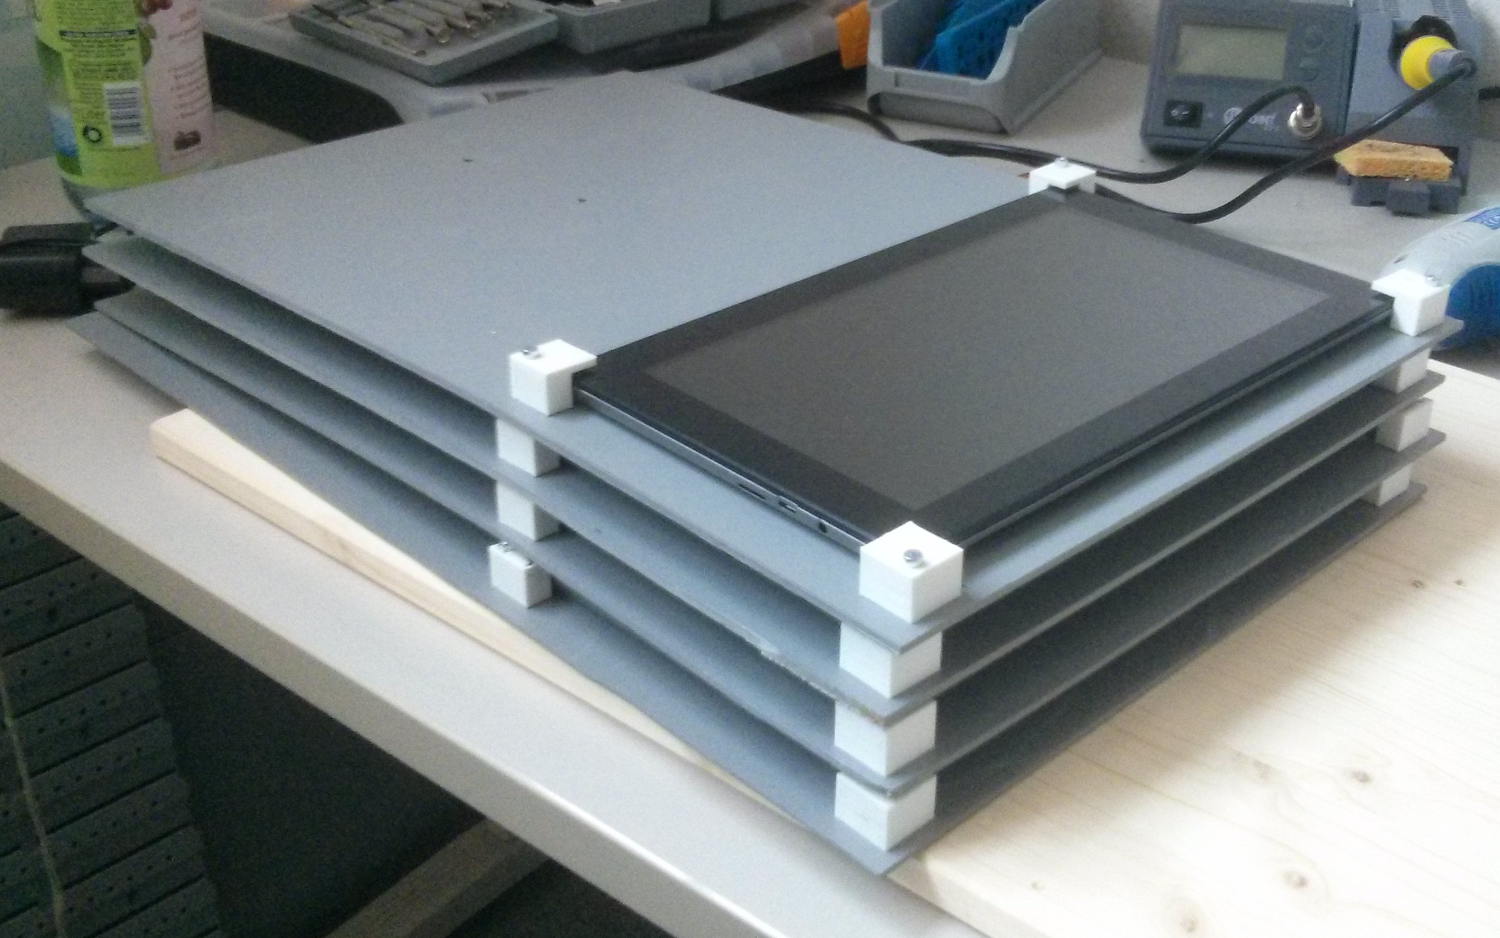
\includegraphics[width=0.85\textwidth]{./img/fertigeAufhaengung.png}
  \caption{Bauhausboards - Aufhängung}
  \label{img:fertigeAufhaengung}
\end{figure}
\\
Damit sich die Testnutzer mit der Grundlegenden Funktion von Bauhausboards vertraut machen konnten, habe ich ein Benutzerhandbuch erstellt.

% Nachdem Umsetzung abgeschlossen war: Test mit echten Nutzern
% Server mit NodeJS und Postfix aufgesetzt
% - Programm auf Server in Uni eingerichtet -> Spezifikationen? oder wurde das schon vorher angegeben?
% - Mailserver installiert, damit Server mails verschicken konnte (nur uni-intern)
% 4 Tablets angeschafft (Durch 4 Tablets -> 4 Räume zum Testen möglich)
%- Blaupunkt Discovery 1000c
%   * 10,1"
%   * CPU: Quadcore @ 1,33GHz
%   * Android 5.1
%   * 1GB RAM
%   * 1024x600 Auflösung (~17:10)
% Alle Tablets mit Kiosk-Mode Browser bestückt
%- Kiosk Mode Browser App auf Tablets um beenden der Bauhausboards App zu verhindern
%- Tasker zum automatischen start des kiosk modes nach systemstart - falls schlaue leute denken, sie können damit den kiosk browser umschiffen
%- Google Locate um Position des Tablets zu bestimmen, im falle eines Diebstahls
%- Rahmen: 4 Tablets -> 4 Räume
%- Wandbefestigung
%  * 3D gedruckte Eckstücke mit Loch um Tablets zu halten + zu sichern
%  * Holz/Blech Rückwand >> plexiglas
%  * Nutzung des vorhandenen Türschildes
%  * Fotos und 3D Model
%- Nutzer Tutorial zur Nutzung des Tools entworfen




\section{Durchführung}\label{Durchführung}
Da nur vier Räume mit Tablets ausgestattet werden konnten, war es von Vorteil, mit den vorhandenen Mitteln möglichst viele Testnutzer organisieren zu können.
Nachdem mehrere verschiedene Leute der Medienfakultät der BUW nach Teilnahme an der Studie gefragt wurden, war es mir möglich einige Mitarbeiter der Professur für Systeme der virtuellen Realität (VR) und der Professur für grafische Datenverarbeitung (CG) zur Teilnahme an der Studie zu bewegen.
\\
Bei der virtuellen Realität gab es drei Büroräume.
Zwei davon mit jeweils drei und einer mit zwei Mitarbeitern.
An der Professur für grafische Datenverarbeitung gab es zwei Mitarbeiter, die sich einen Raum teilten.
Diese Räume befanden sich alle im selben Gang der Fakultät.
\\
Da ein Mitarbeiter der VR Professur durch seine Forschungsarbeit nicht in seinem Büro sein konnte, nahm er nicht an der Studie teil.
\\
Somit konnten insgesamt 9 \todotext{Doktoranden und wie heißen die fertigen Doktoranden?} Testnutzer organisiert werden.
\\
\\
Bevor die Studie beginnen konnte, mussten die Boards angebracht werden.
\\\todotext{Bild von aufgehängten Boards}\\
Außerdem musste eine gute WLAN Verbindung für sie gewährleistet sein.
\\\todotext{Grundriss des Gangs mit Tablets + Accesspoint}\\
Nachdem die Boards aufgehangen waren, wurde für jeden Benutzer ein Account erstellt, die Boards eingerichtet und die Nutzer kurz eingewiesen.
\\
Die Dauer der Studie beschränkte sich auf zwei Wochen.
Damit sollte mindestens ein Wochenende mit eingeplant sein, da sich das Benutzerverhalten nach diesen zwei Tagen ändern konnte.
\\
Während der Studie kam es von Zeit zu Zeit dazu, dass einige Testnutzern Fragen zu bestimmten Funktionen hatten, welche direkt geklärt wurden.
Das System wurde gut genutzt und einige Gäste hinterließen den Testern Nachrichten.



\section{Auswertung}\label{Auswertung}
Nach Abschluss der Studie sollten alle Teilnehmer Interviewt werden.
Dazu musste vorher ein Fragenkatalog erstellt werden, um von den Testnutzern Feedback zu den wichtigsten Funktionen des Systems zu erhalten.
\\\todotext{mehr}
\subsection{Interview}\label{Interview}
%- Aufnahme des Interviews (Audiofile)
% 330min Interview = 5h30min
% Aufteilung in Nachrichten empfangen, Nachrichten schreiben, Statusmeldungen, Nutzerinhalte, Editor, Boardfunktionen, Allgemeines
\subsubsection{Nachrichten empfangen}\label{Nachrichten Empfangen}
% Nachrichten empfangen
%  - mit den Nutzern die empfangenen Nachrichten durchgegangen um Herauszufinden, wofür die Gäste die Funktion genutzt haben
%  - Größtenteils keine ernst gemeinten Nachrichten (Spaßnachrichten, ``temporäres Grafitty'')
%  - ab und an Fragen, ob man zusammen Mittag essen gehen will oder ob Nutzer zugegen ist

%  - es war in keiner Nachricht ersichtlich, wer deren Autor war
%  - wurde von den Meisten Testnutzern bemängelt, dass sie den Autor nicht identifizieren konnten (sie konnten nur ab und an vermuten, wer es war)

%  - Nutzer wurden gefragt, wie man ihnen sonst eine Nachricht hinterlassen konnten
%  - die meisten meinten: per mail
%  - aber auch: postIt, tel, klopfen, sms(dafür müssen aber kontaktdaten da sein), usw

%  - Nutzer gefragt, ob es für sie anders war, über das Board eine Nachricht zu erhalten
%  - war praktisch, ``Die Zeichnung macht es anders'' (also positiv, dass Zeichnungen drin waren) es schafft eine persönliche Note, aber für manche war es nicht anders als eine normale mail(und demnach gut)

% - Alle haben dadurch, da sie per mail benachrichtigt wurden, es direkt gelesen, da sie auch direkt auf den link in der mail klicken konnten und sich deswegen nicht extra anmelden mussten

% - einige Nutzer fanden es gut, dass man ihnen eine Nachricht hinterlassen konnten, wenn sie grade nicht im Büro waren
% - als größtes Manko empfanden die Testnutzer, dass sie nicht sehen konnten, wer die Nachricht geschrieben hat
% - andere fanden es zu umständlich, einen einfachen text einzugeben, da die Touchauflösung des Tablets zu gering war
% - außerdem wurde es gut aufgenommen, dass man für die KOmmunikation mit den Besitzern nicht extra ein eigenes Gerät brauchte, da die Boards vor den Büros hingen

% - Verbesserungsvorschläge: autorkennzeichnung, voicemail, videomail, Vordefinierte Nachrichtenkategorien(dem Anliegen entsprechend), Vereinfachung durch weniger untermenüs
%%%%%%%%%%%%%%%%%%%%%%%%%%%%%%%%%%%%%%%%%%%%%%%%%%%%%%%%%%%%%%%%%%%%%%%%%%%%%%%%
\subsubsection{Nachrichten schreiben}\label{Nachrichten schreiben}
% selber Nachrichten schreiben
% - Auf die Frage, ob die Testnutzer einem anderen Besitzer eine Nachricht auf ihr Board hinterlassen haben, meinten die meisten, dass sie selber nur die Besitzerrolle wahrgenommen hatten und keinem eine Nachricht hinterlassen haben
% - das hatte den Grund, da sich die meisten Tester persönlich sehr gut kannten und die meiste Kommunikation mündlich durchführten
% - Einem Nutzer war der ganze Nachrichtenprozess zu viel Aufwand (und es war ihm zu versteckt)
% - ein paar Testnutzer nutzen es, um einen anderen Nutzer zu fragen, ob er mit zum Mittagessen mitkommen wollte
%%%%%%%%%%%%%%%%%%%%%%%%%%%%%%%%%%%%%%%%%%%%%%%%%%%%%%%%%%%%%%%%%%%%%%%%%%%%%%%%
\subsubsection{Status}\label{Status}
% Statusfunktion
% - die meisten Testnutzer haben die Funktion direkt genutzt oder aber sich ihren Status auf ihre Pinnwand geschrieben
% - davon haben alle Nutzer bis auf einen die Funktion vom PC aus genutzt, der andere wollte es am Board ändern, war aber der meinung, dass es für ihn zu kompliziert war, den status zu ändern (der meinung waren auch einige andere Testnutzer)
% - übliche Statustexte waren: ``busy'' oder ``im DBL zu finden'' oder im Meeting oder ganz einfach N/A
% - wie gesagt einige fanden das system zu kompliziert, vorallem das Interface (es bot zu viel auf einmal und war zu schwer zu erreichen)
% - andere wiederum fanden es gut, dass es dieses feature gab und man gesondert seinen aktuellen status kennzeichnen konnte
% - nützlich für gäste, um zu wissen, wann der Besitzer wieder da ist
% - Kollegen von Testnutzern mussten nicht wegen dessen status behelligt werden 
% - die meisten Nutzer haben den Status vor dem Verlassen des Büros geändert, wenn sie essen gegangen sind oder ins Meeting
% - auf die Frage ob Vordefinierte Status sie eher dazu animieren würden, das Feature zu nutzen meinte die Mehrzahl, dass es das würde

% - Die Auswertung ergab, dass die N/A Funktion zum Ausgrauen des Nutzerbildes nicht gebraucht wird

% - viele meinten, dass der Status zu unoffensichtlich ist und besser gekennzeichnet werden müsste oder komplett heraus genommen werden sollte, da man das auch alles über den COntent machen könnte
% - Ein Nutzer meinte, er würde seinen Status nur von unterwegs ändern, wenn er dem system eine mail mit dem statustext schicken könnte oder es per app machen könnte
% - Die Funktion sollte komplett vom Board genommen werden und nur für die Desktop-Version zugägnlich sein

% - der grund warum einige das Feature nicht genutzt haben war, dass ``sie eh die ganze Zeit da waren und es deswegen nicht brauchten'' oder es nicht für nötig hielten, da eine geschlossene Tür schon statusindikator genug ist ``Wenn die Tür zu ist, bin ich nicht da''
%%%%%%%%%%%%%%%%%%%%%%%%%%%%%%%%%%%%%%%%%%%%%%%%%%%%%%%%%%%%%%%%%%%%%%%%%%%%%%%%
\subsubsection{Nutzerinhalt}\label{Nutzerinhalt}
% Content ändern
% - der Content wurde hauptsächlich für spaß benutzt, es wurden Bilder und gifs hochgeladen und präsentiert. Aber es wurde auch zum Teil zur präsentation von fachlichem Inhalt verwendet ``um von außen einen schnelleren Eindruck zu gewähren, was ich mache''
% - andere Nutzen diese Funktion wie schon gesagt zur ANzeige ihres Status

% - entweder wurde der Editorlayer oder aber der Backgroundlayer zur Anzeige von Bildern/Gifs genutzt weil es war für die NUtzer nicht offensichtlich, wie man im Editorlayer bilder hochlädt --> einbau eines buttons dafür
% - genutzt für Webseiten (Nachrichten oder Seite der Professur)
% - Backgroundlayer wurde größtenteils positiv aufgenommen, wäre aber besser als poweruserfunktion
% - ein Nutzer meinte: Nutzer sollten selber über Background-Interaktivität entscheiden können

% - alle Nutzer haben nicht das twitterfeature genutzt, da fast alle keinen twitteraccount hatten
% - der eine Nutzer, der einen acc hatte, würde das feature nicht nutzen, da er privaten inhalt sonst präsentieren müsste

% - NUtzer fanden es interessant, da technologie neu war, man bewegten Inhalt präsentieren konnte oder einfach nur aus spaß
% - die nutzer, die es nicht benutzten hatten entweder keine Zeit einen content zu erstellen oder ihnen ist nichts eingefallen

% - übliche änderungszeit war zur Mittagszeit in der pause
% - leider ist benutzung mit der zeit eingeschlafen (nur am anfang der studie, danach weniger genutzt)

% - schön war es, dass es ab und an auch gäste gab, die auf den content von besitzern eingegangen sind und ein gespräch deswegen entstanden ist

% - von den meisten wurde es positiv aufgenommen: der persönliche Aspekt ``Sehr gut war die Möglichkeit selber Kreativ zu werden''
% - auch gut war es, dass man damit INformationen präsentieren konnte
% - am besten fanden die TEster, dass man damit gifs anzeigen konnte

% - einige Benutzer fanden wieder die bedienung zu kompliziert und, dass es zu viele features gab, dass man es auch hätte vereinfachen können
% - zu viele schritte, bis content geändert wurde --> weniger klicks desto besser

% - es wäre wahrscheinlich ernster benutzt worden, wenn es ganz offiziell da hängen würde oder es kommuniziert worden wäre, für welchen Content es vorrangig genutzt werden sollte
%%%%%%%%%%%%%%%%%%%%%%%%%%%%%%%%%%%%%%%%%%%%%%%%%%%%%%%%%%%%%%%%%%%%%%%%%%%%%%%%
\subsubsection{Editor}\label{Editor}
% Editor Benutzung
% - fast alle (außer 2) haben den Editor benutzt
% - sie haben es dafür benutzt um bspw eigene Arbeit zu skizzieren, texte zu zeichnen oder einfach nur spaßzeichnungen zu machen
% - die anderen meinten die benutzung wäre zu versteckt im backend
% - da die icons nicht wie in den üblichen editoren waren, waren sie nicht eindeutig(color=underline,selector wie rectangleZeichnen,undo-redo->geschwungene pfeile)
% - einigen war nicht von anfang an bewusst, dass sie bilder und gifs per drag and drop einbinden können (sie benutzten dafür die hintergrundlayer) -> musste ihnen erst gezeigt werden   ---> lieber Hinweis auf Funktion machen + extra upload button
% - es war schlecht, dass es keine autoskallierung für bilder und keine vordefinierten formen gab
% - außerdem wurde es bemängelt, dass das ausgewählte werkeug zu wenig hervorgehoben wurde

% - positiv war, dass er recht intuitiv zu benutzen war, dass er postIt ähnlich war

% - ``Es war für den Rahmen in dem es lief ausreichend''
% - ein Nutzer meinte, dass das schon allein als Boardfeature reichen würde
% - ausmalfeature wäre noch gewünscht
% - wekzeuge sollten dauerhaft angezeigt werden
%%%%%%%%%%%%%%%%%%%%%%%%%%%%%%%%%%%%%%%%%%%%%%%%%%%%%%%%%%%%%%%%%%%%%%%%%%%%%%%%
\subsubsection{Boardfunktionen}\label{Boardfunktionen}
% Allgemeine Boardfunktionen
% - es war für einige Tstnutzer nicht ersichtlich, wo sie sich im backend befanden, ob sie noch angemeldet sind und wer überhaupt angemeldet ist
% - deswegen sollte lieber das BAckend vom Frontend getrennt werden und vereinfachen (da jetzt zu viele klicks notwendig waren)
% - Alle Nutzer waren der Meinung, dass 2 Authentisierungen übertrieben sind
% - wenn Frontend und Backend getrennt wären, bräcuhte man nur eine Authentisierungsmethode
% - ein Nutzer war sogar der Meinung Passwortauthentisierung komplett weg zu lassen ``auch wenn es Vandalismus Tür und Tor öffnet''

% Frage, was sie als Vor- und Nachteile gegenüber PostIts, Whiteboards und Pinnwänden sehen
% positiv:
% - digitaler/dynamischer content
% - produziert keinen müll
% - die Besitzer werden direkt über Nachrichten informiert(per mail)
% - privacy(nur empfänger kann nachricht lesen)
% - keiner kann Nachricht löschen - postIt/whiteboardnachrichten aber entfernbar
% - Erstellung von Content per Remote
% - Kontaktaufnahme, selbst wenn Kontaktdaten unbekannt oder man kein geeignetes device zur hand hat
% - macht spaß
% - daten werden archiviert

% negativ
% - kostet energie
% - teurer als postIts
% - wird nur als spielerei wahrgenommen + Statusmeldungen im endeffekt nur peripher von Gästen wahrgenommen (postIts werden ernster genommen)

% - Die Größe der Boards fanden alle angemessen und hätten nicht unbedingt größere Boards gebraucht

% - viele waren der Meinung, dass der Wechsel zwischen den Benutzern nervig war
% - sie hätten lieber gewollt, dass die Nutzer parallel angezeigt werden, sodass man dann direkt auf den Benutzer klicken könnte um ihn eine Nachricht zu schreiben
% - dadurch hat man auch eine direkte sicht darauf, wer alles im Raum arbeitet, wer davon grad nicht verfügbar ist und was so dessen Status ist
% - dafür wäre auch in Kauf genommen, dass nur 1/3 Platz für Content zu Verfügung steht


%%%%%%%%%%%%%%%%%%%%%%%%%%%%%%%%%%%%%%%%%%%%%%%%%%%%%%%%%%%%%%%%%%%%%%%%%%%%%%%%
\subsubsection{Allgemeine Anmerkungen}\label{Allgemeine Anmerkungen}
% Allgemeine Anmerkungen
% - Studie war zu kurz um sich wirklich dran zu gewöhnen, weswegen die Funktionalität nicht in den Arbeitsprozess mit eingegangen ist
% - Teilweise waren die Menüpunkte nicht eindeutig bezeichnet
% - ``es war schön, dass man darüber Nachrichten empfangen konnte''
% - Für einen Testnutzer war es zu viel Aufwand, wenn man etwas auswählen musste oder durch das menü navigieren musste ``Keiner möchte ewig vor seinem Büro stehen und da rum klicken'' --> deswegen Trennung Frontend/Backend
% - Am besten wäre für zusätzliche Funktionalität eine Poweruser Einstellung
% - ein Nutzer meinte die Boards sind gute Notleuchten und dass sie gute Blickfänger sind
%%%%%%%%%%%%%%%%%%%%%%%%%%%%%%%%%%%%%%%%%%%%%%%%%%%%%%%%%%%%%%%%%%%%%%%%%%%%%%%%





% Ergebnisse der Interviews
%   * manche Nutzer haben nichtmal das Tutorial gelesen ...
%   * Großteil der Nutzer meinte, dass es unersichtlich ist, wer alles im Raum arbeite und es besser wäre, dass man auf den ersten Blick erkennen könnte, wer alles drin arbeitet (sowas wie Nutzerliste Rechts unter Header)
%   * Ein Bug wurde entdeckt, dass wenn man noch keinen Content eingestellt hatte und man dann einen Hintergrund setzen will man ausgeloggt wird, da eine exception geschmissen wurde (Lösung eigene Background Tabelle in der DB)


\subsection{UEQ Fragebogen}\label{UEQ Fragebogen}






% UEQ Fragebogen nach Testlauf
% was ist UEQ
% Ergebnisse des UEQ